\section{Theorie}
\label{sec:Theorie}

Brückenschaltungen werden im Allgemeinen dazu verwendet Widerstände zu messen.
Dies ist nützlich, da sich einige physikalische Größen durch den Widerstand ausdrücken lassen, zum Beispiel die Temperatur.
Außerdem können spezielle Brückenschaltungen Frequenzen filtern, was sie auch in der Mess- und Kommunikationstechnik wichtig macht.

Für den Grundsätzlichen Aufbau einer Brückenschaltungen werden vier Widerstände benötigt.
Diese werden mit einer Speisespannung $U_S$ gespeist. Dabei werden jeweils zwei der Widerstände in Reihe geschaltet.
Diese In Reihe geschalteten Widerstandspaare werden dann wiederum parallel geschaltet wie in \ref{fig:brueckprinzip} zu sehen ist.

\begin{figure}
    \centering
    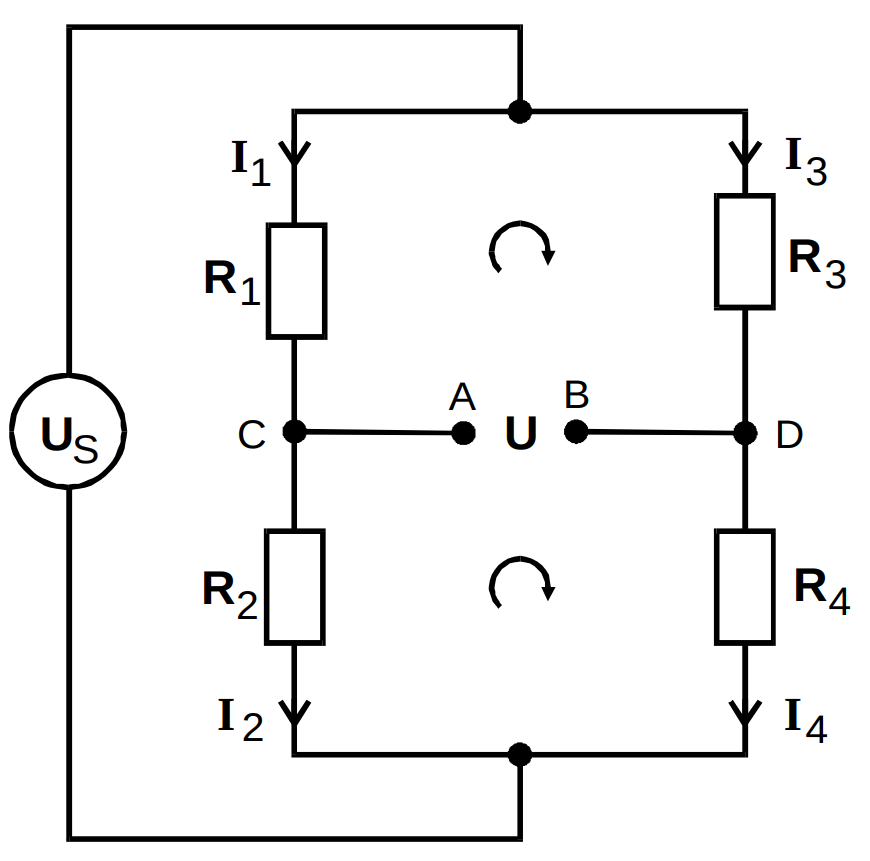
\includegraphics[scale=0.25]{content/Brueckenschaltung.png}
    \caption{Eine prinzipielle Brückenschaltung. \cite[S. 216]{anleitung}}
    \label{fig:brueckprinzip}
\end{figure}

Daraufhin lässt sich ziwschen Punkt $A$ und Punkt $B$ eine Brückspannung $U_B$ abgreifen.
Mit Hilfe der beiden Kirchhoffschen Gesetzte
\begin{enumerate}
\item Die Summe alle zufließenden und abfließenden ströme ist gleich Null:
\begin{equation}
\sum_k I_k = 0
\end{equation}
\item Die Summe aller Spannungen in einem Knoten nach Beachtungen der Vorzeichen gleich Null:
\begin{equation}
\sum_k U_k = 0
\end{equation}
\end{enumerate}
ergibt sich dann für die Brückspannung 
\begin{equation}
U_B = \frac{R_2\cdot R_3 - R_1 \cdot R_4}{(R_3 + R_4) \cdot (R_1 + R_2)} \cdot U_s .
\label{eqn:Brueckspannung}
\end{equation}
Wenn nun die Widerstände $R_3$ und $R_4$ so gewählt werden, dass die Brückspannung verschwindet,
ergibt sich aus \eqref{eqn:Brueckspannung} die sogenannte Abgleichbedinnung:
\begin{equation}
R_2 R_3 = R_1 R_4 .
\label{eqn:abgleich}
\end{equation}
Dabei ist es egal ob komplexe oder reele Widerstände verwendet werden, darauf wird allerdings später nocheinmal eingegangen.

\subsection{Wheatstonesche Brücke}

\begin{figure}
    \centering
    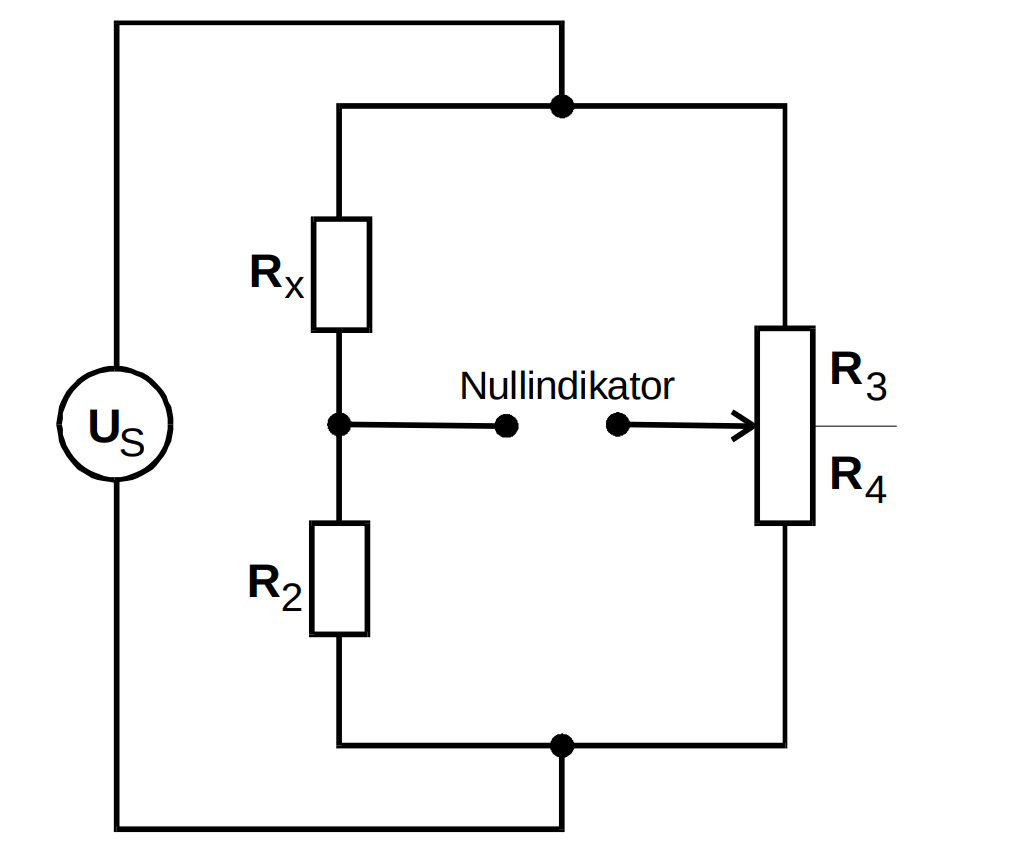
\includegraphics[scale=0.25]{content/Wheatstonesche.png}
    \label{fig:wheatstonesche}
    \caption{Die Wheatstonesche Brücke \cite[S. 219]{anleitung}.}
\end{figure}

Anstatt fester Widerstände wird nun für $R_3$ und $R_4$ ein Potentiometer verwendet.
Außerdem werden nur ohmsche Widerstände verwendet, von denen der Widerstand $R_x$ unbekannt ist.
Dieser kann ermittelt werden indem \eqref{eqn:abgleich} nach $R_x$ umgestellt wird:
\begin{equation}
    R_x = R_2 \frac{R_3}{R_4}.
\end{equation}

\subsection{Kapazitätsmessbrücke}

\begin{figure}
    \centering
    \includegraphics[scale=0.25]{content/Kapazitätsmessbruecke.png}
    \label{fig:kapa}
    \caption{Die Kapazitätsmessbrücke \cite[S. 220]{anleitung}.}
\end{figure}

